% Chapter 1

\chapter{Experiments} % Main chapter title

\label{Chapter8}

In this chapter we display a novel usage of our new the $ID$ attributes and qualities.

Here we will use our $ID$ method in order to obtain a perceptual colors distance metric learning, which is a high demanded function in computer vision region. Our examination is based and referring to \cite{perp_color} paper, which developed a local metric embedding method for this problem. 

This set of experiments tries to adapt a perceptual color difference metrics, based on various color samples originated from several cameras, angles, illuminations etc.
\\

Our $ID$ method would be examined in this section solely by the original experiment's accuracy measures - Mean Absolute Error \cite{MAE} and STRESS \cite{STRESS}
\\
Further discussion will refer to the various exams may apply on our $ID$ method according to our described theory.

\section{Experiment Procedure}



\textbf{object pairs ID embedding} \ref{Chapter3} will be demonstrated by applying its embedding method over pairs which was taken and labeled from the Farnsworth-Munsell 100 hue-test set \cite{furnsworth}.
\subsection{Dataset}

Dataset of this experiment is assembled from single color patches, which displayed in a set of images, where each image was generated by a specific set of image features, such illumination, camera type (4 different cameras are involved in the dataset creation) , lance type , background etc.

\begin{figure}[h] \label{set_ds}
			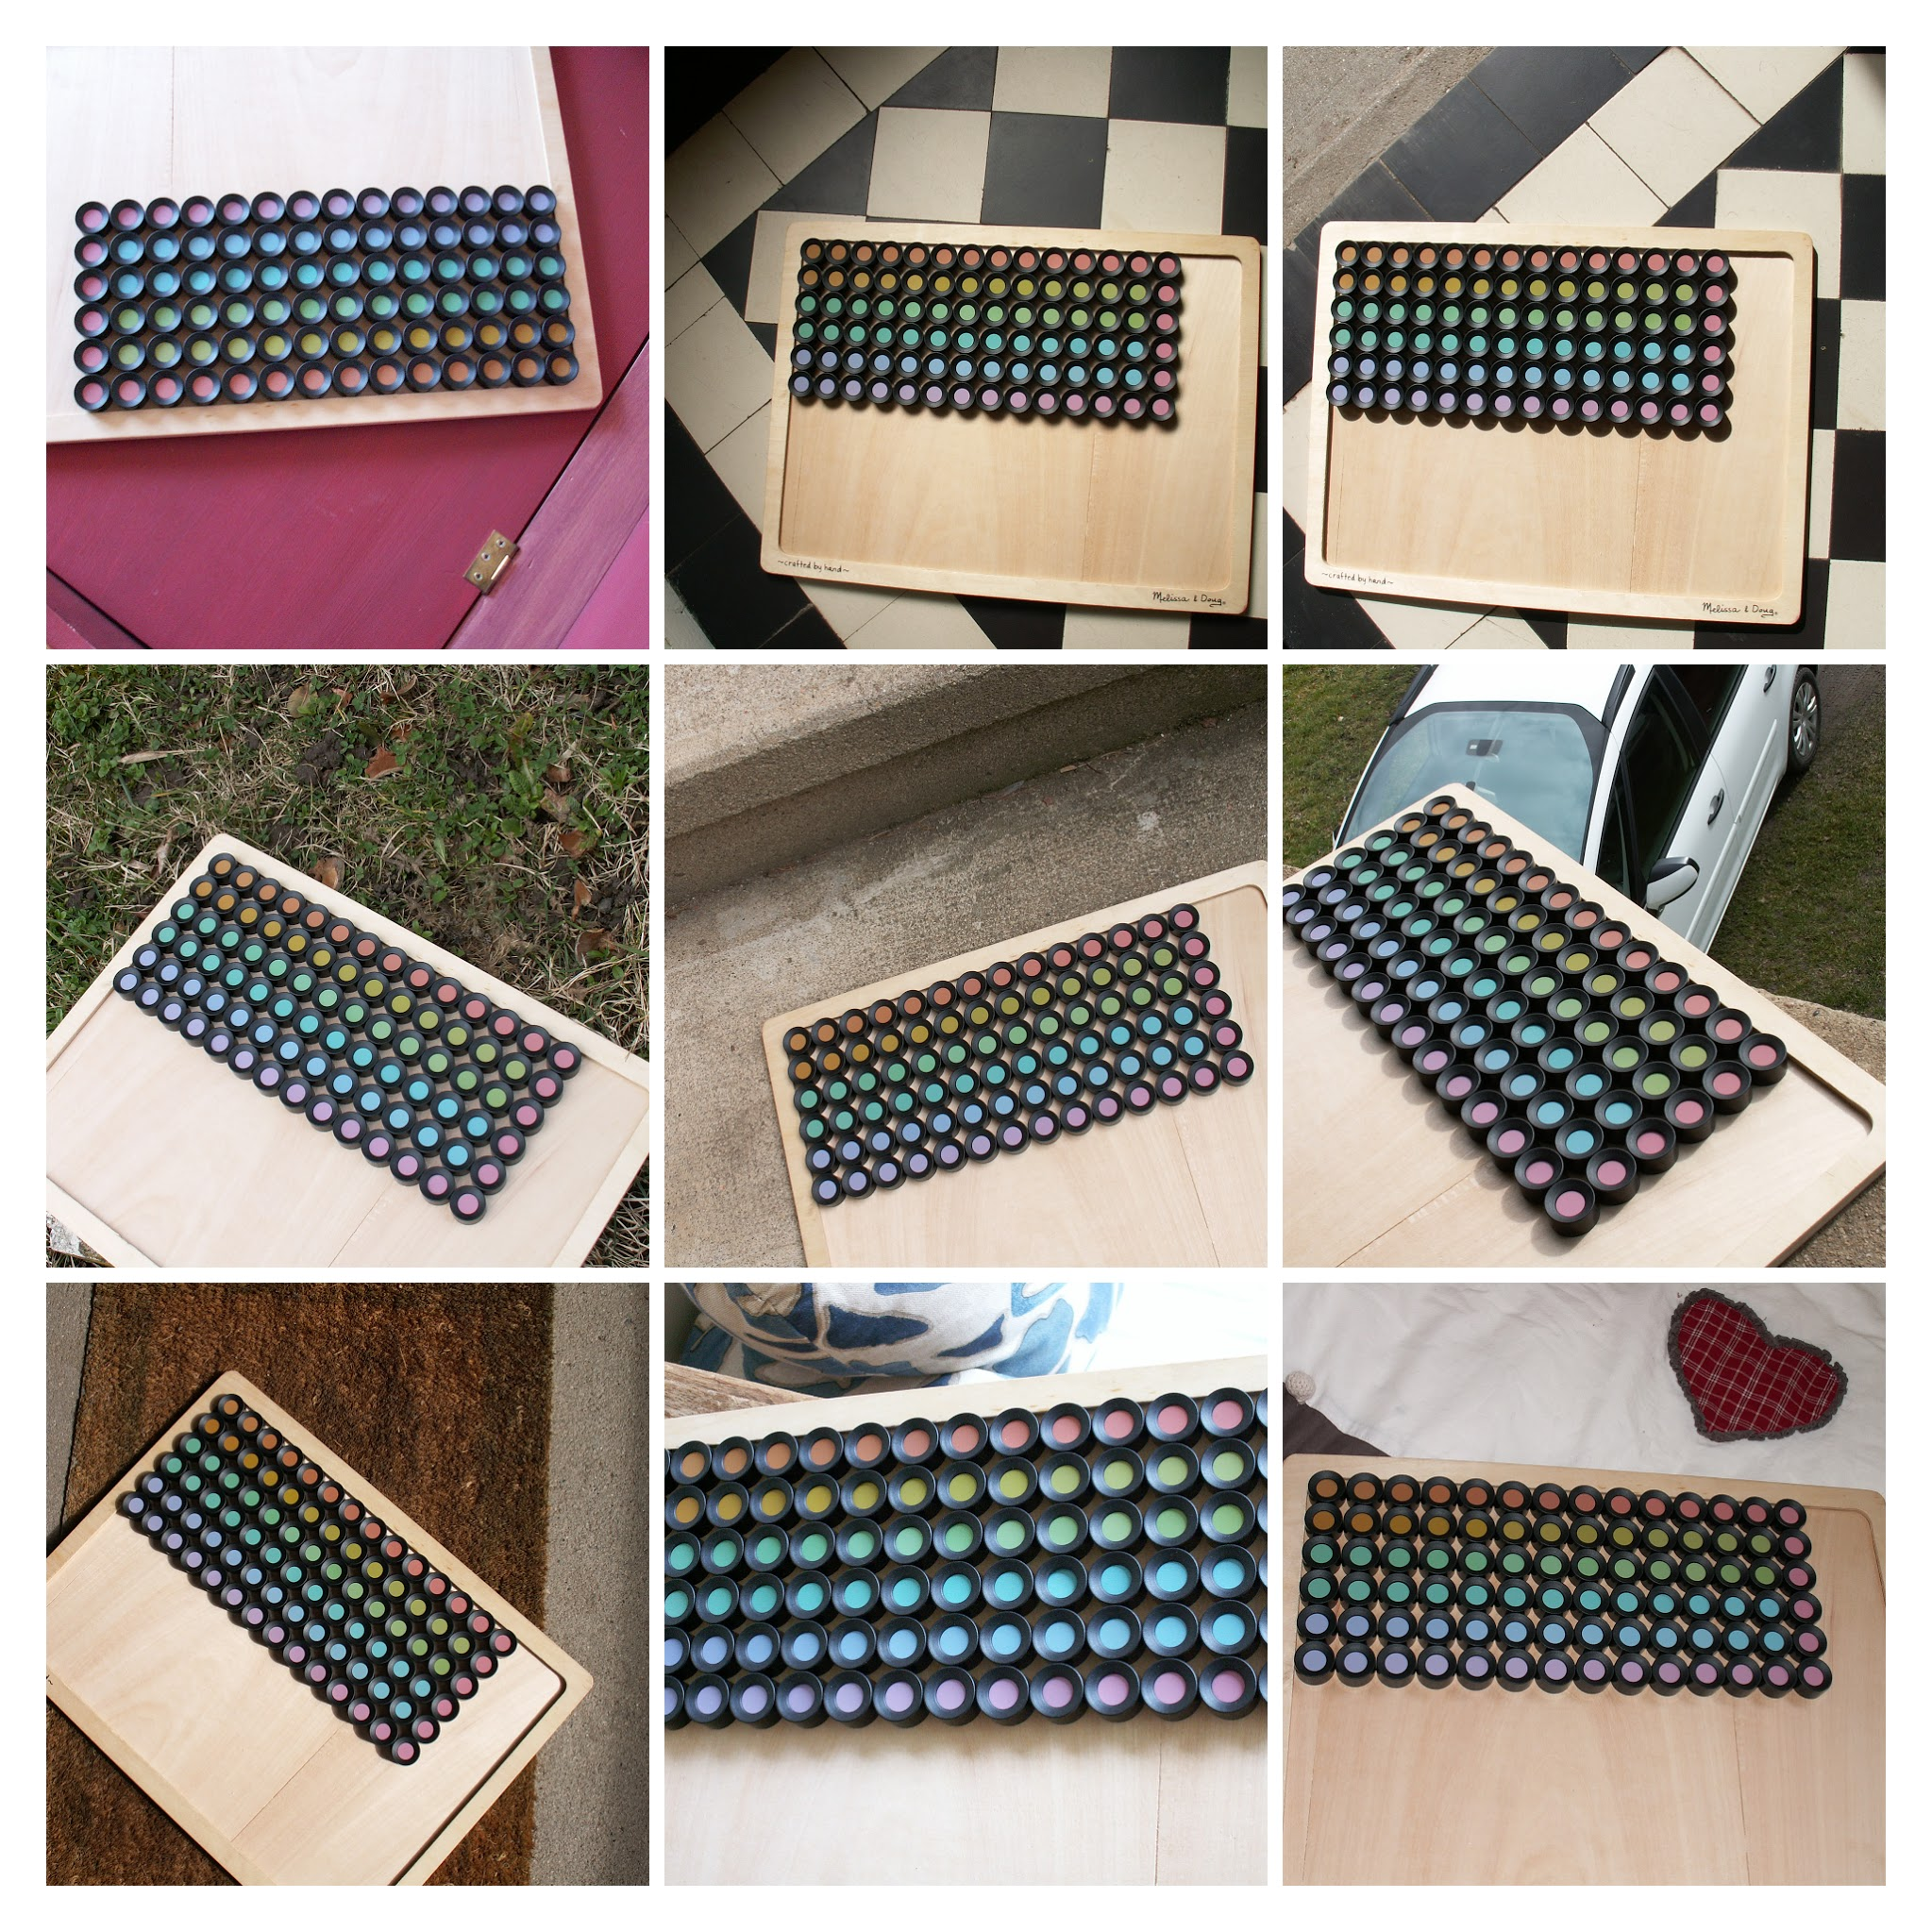
\includegraphics[width=\linewidth,height=12cm,keepaspectratio]{Figures/set_ds}
			\caption[set ds]
			{set ds}
\end{figure}

For each color patch, a $L^*A^*B^*$ \cite{lab} coordinates are given. 
Since the pairs of patches should be close by their CIELAB \cite{CIELAB} coordinates in order to adapt a good color difference assessment, a set in the final dataset is only a set of patches, where its CIELAB euclidean distance is relatively close, i.e. $\Delta E \leq 5$ .


\begin{figure}[h] \label{patch_positions}
			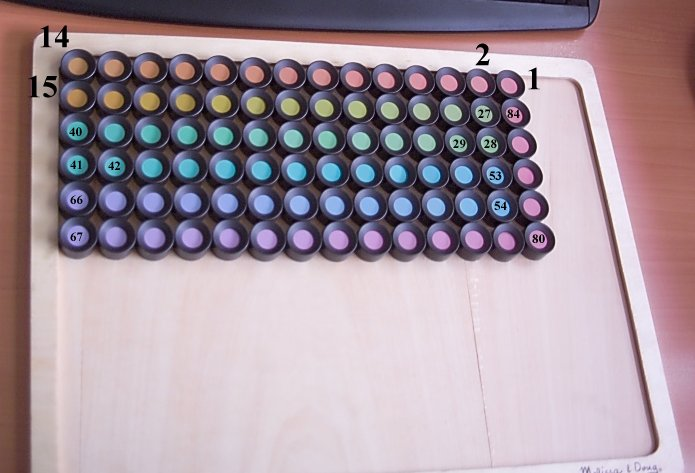
\includegraphics[width=\linewidth,height=12cm,keepaspectratio]{Figures/patch_positions}
			\caption[patches order]
			{patches order}
\end{figure}


\subsection{Models to train}
Then, $ID$ learning method will try to learn some similarity models according to a couple of test conditions:

\begin{itemize}
	\item \textbf{unseen colors} - dividing the entire patches set into train-test sets
	\item \textbf{unseen cameras} - assigning 3 out of 4 cameras sets as train set, and make the remained camera set as test set. \\
		training set cameras:
		\begin{itemize}
			\item Kodak DCS	Pro 14n
			\item Konica Minolta Dimage Z3
			\item Nikon Coolpix S6150
		\end{itemize}	
		
		test set camera:	
		\begin{itemize}
			\item Sony DCR-SR32
		\end{itemize}
		
\end{itemize}

\subsection{Interpolation}
Data dimension in our scenarios is of course $n=3$ (for lab/RGB \cite{RGB} coordinates), and for an object pair the dimension is $2n=6$. \\
As described in \ref{Chapter3}, interpolation is performed dimension-wise along the training set, after selecting data center per dimension by manual/automatic method.
\\
In our experiment we have selected an automatic cross validation \cite{cross validation} method for assessing the optimal number of centers per dimension, and find those by using k-means \cite{kmeans} algorithm.
\\
For this number of extracted centers we add 2 extreme points for applying proper interpolation for data values beyond limits of the discovered centers.
\\
Now that we have found data centers for each dimension we apply our interpolation method \ref{interpolation pairs} on our data (on both train-test sets) and extract a $\overrightarrow{a} \in \Re^6$ coefficient vector per color patches pair, which is ready to be embedded.


\subsection{Embedding}
Embedding is performed by applying an embedding of the coefficient vectors on a sparse form such $\overrightarrow{e} \in \Re^{\prod_{i=1}^{2n}{length(\overrightarrow{c_i})}}$ , where $n = 3$.
Each coefficient vector element is assigned to the exact simplex index in the $\overrightarrow{e}$ embedded vector.
\\
For memory savings, we have performed a reduction to all columns along the entire dataset, where all elements were equal to zero.
Since our embedded vectors are sparsed, it was quite common to have over $90 \% $ of the samples elements to be total zeroed so final actual dimension of our sets were almost always $ \le 100$ .

\subsection{Learning}
Learning is performed as a linear regression model training.
We learn by using SGD \cite{SGD} learning algorithm, and with a MSE \cite{MSE} loss function.
We also applied a standard Tichonov \cite{Tichonov} regularizer on the learning process as described in the learning chapter \ref{Chapter6}.


\subsection{Assessment}
Assessment is operated following two criterias:
\begin{itemize}
\item \textbf{MAE} - Mean Absolute Error
\item \textbf{STRESS} - Standardized Residual Sum of Squares \cite{STRESS} \\
\end{itemize}

MAE index is measured as:
\begin{equation}
MAE = \frac{1}{n} \cdot \sum_{i = 1}^{n}{|y^{pred}_i - y^{test}_i|}
\end{equation}

Where n is dataset size. \\

STRESS index is measured as follows:
\begin{equation}
STRESS = \sqrt{100 \cdot \dfrac{\sum\limits_{i}{(y^{pred}_i - F \cdot y^{test}_i)^2}}{\sum\limits_{i}^{}{F^2 \cdot (y^{test}_i)^2 }}}
\end{equation}

Where F factor is assembled as:
\begin{equation}
F = \dfrac{\sum\limits_{i}{(y^{pred}_i)^2}}{\sum\limits_{i}{y^{test}_i \cdot y^{pred}_i }}
\end{equation}







\section{Results}

we now describe our results as compared to the original paper results as described in \ref{original paper results}


\subsection{Unseen Colors}

Unseen camera case was assembled by a certain percentage of all data set as train set, and the rest as test set. In this experiment we have taken the train set size to be $80 \%$ of the total data set.
		
		\subsubsection{Dataset properties}
		
			From a total 13500 patches pairs set, the divided train-test sets amounts are:
			\begin{itemize}
				\item \textbf{train set size} = $10800$ 
				\item \textbf{test set size} = $2700$
			\end{itemize}
			
			train/set ratio = $4/1$
			
		\subsubsection{Centers locations}
		
		Centers locations are shown as extracted via cross-validation for finding optimal number of centers per dimension, and k-means for extracting centers values. \\
		k-means actually found only the inner centers, since the outer centers are fixed bounds.\\
		
		$\begin{matrix}  \qquad  c_0 \quad  \qquad c_1 \quad  \qquad c_2 \qquad \quad  c_3 \qquad \quad c_4 \qquad \quad c_5 \quad \end{matrix}\\
				
		
		\begin{pmatrix}
				     -0.01 &     -0.01 &    -0.01 & -0.01   & -0.01   & -0.01   \\
					100.78 &   116.35 &    81.09 &    100.02 & 116.53 & 93.74   \\
					153.59 &   140.96 &   97.78 &   159.02 & 144.20 & 136.93    \\
					       &          &  114.13 &          &        &           \\
					       &          &   131.81 &          &        &          \\				       
					       &          &   151.10 &          &        &          \\				       
		     		 255.01 &  255.01 &   255.01 &   255.01 &  255.01 &  255.01 & \\
				\end{pmatrix}$\\
$ $

		In this scenario, there are 4 extracted centers per dimension besides the $3^{rd}$ one, which has 7 extracted centers. This difference may be since its ($3^{rd}$ dimension of the paired vector) variance is much higher than the rest.

	\subsubsection{Experiment Figures}
	
	Our model provides the following figures:

	\begin{itemize}
	\item 	p-value = $3.9 \cdot 10 ^{-03}$
	\item 	STRESS = $26.62$
	\item 	MAE = $0.80$
	
	\end{itemize}


\subsection{Unseen Camera}

Unseen camera scenario was assembled by assigning one of the cameras involved in dataset generation as test set, where the other 3 functions as train set.


	\subsubsection{Dataset properties}
	
		From a total 13500 patches pairs set, the divided train-test sets amounts are:
		\begin{itemize}
			\item \textbf{train set size} = $8084$ 
			\item \textbf{test set size} = $5416$ (Sony DCR-SR32 camera set)
		\end{itemize}
		
		train/set ratio = $3/2$

	\subsubsection{Centers locations}
	
	Centers locations are shown as extracted via cross-validation for finding optimal number of centers per dimension, and k-means for extracting centers values. \\
	k-means actually found only the inner centers, since the outer centers are fixed bounds.


	$
	\begin{matrix}  \qquad  c_0 \quad  \qquad c_1 \quad  \qquad c_2 \qquad \quad  c_3 \qquad \quad c_4 \qquad \quad c_5 \quad \end{matrix}
			
	
	\begin{pmatrix}
			     -0.01 &     -0.01 &    -0.01 & -0.01   & -0.01   & -0.01    \\
				100.46 &   116.35 &    82.81 &    95.72 & 115.95 & 88.81     \\
				153.96 &   140.96 &   126.01 &   159.54 & 143.60 & 143.38    \\
				       &          &   147.80 &          &        &             \\
	     		 255.01 &  255.01 &   255.01 &   255.01 &  255.01 &  255.01 & \\
			\end{pmatrix}
	$ 
\\
$ $
	

	As seen in centers list, edges are equal per dimension $[-0.01 , 255.01]$ for data bounding.\\
	
	\subsubsection{Experiment Figures}	
	Our model provides the following figures:	
	\begin{itemize}
	\item 	p-value = $4.5 \cdot 10 ^{-05}$
	\item 	STRESS = $25.59$
	\item 	MAE = $0.79$
	
	\end{itemize}

\subsection{Comparison}

\begin{figure}[h] \label{original paper results}
			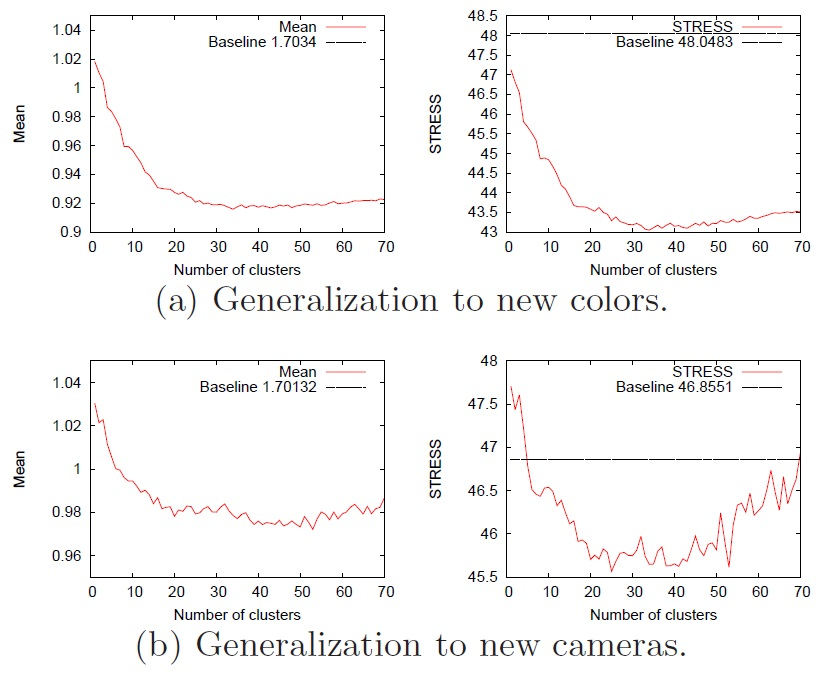
\includegraphics[width=\linewidth,height=12cm,keepaspectratio]{Figures/original_paper_results}
			\caption[orig res]
			{Generalization of the learned metrics to new colors; (b) Generalization of
			the learned metrics to new cameras. For (a) and (b), we plotted the Mean and STRESS
			values as a function of the number of clusters. The horizontal dashed line represents
			the STRESS baseline of $\Delta E_{00}$ . For the sake of readability, we have not plotted the
			mean baseline of $\Delta E_{00}$ at 1.70.}
\end{figure}


Let us treat our results versus the original paper's results.\\

While \cite{prep_color} (regression) method


\ref{original paper results} shows results for either camera/color scenarios, for both model assessment tools - MAE, STRESS. \\
The \ref{original paper results} charts' x - axes describes the number of clusters been used in their embedding algorithm. \\
Their minimal values on both scenarios\textbf{ are > 0.9 for MAE and > 40 for STRESS}, where our results \textbf{ are < 0.85 for MAE and < 30 for STRESS}, all for a $p - value$ with a similar magnitude to theirs. \\
As clearly seen, our results applies the following conditions:
\begin{itemize}
\item Outperforming reference original paper error scores
\item Small p-values which proves the validity of our method, since there is a reasonable assumption that our models provide close dataset approximation
\end{itemize}

This information officially confirms the assumption that our method is valid to work with in terms of reliability. In the following chapter we will discuss the further explorations should be performed to examine the rest of performance criterias mentioned above.





